% ICASSP 2027 working draft. Official template files live in ../template.
\documentclass{article}
\usepackage{../template/spconf,amsmath,amssymb,graphicx}
\usepackage{booktabs}
\usepackage[table]{xcolor}

\newcommand{\obs}{\mathrm{obs}}
\newcommand{\phy}{\mathrm{phy}}
\newcommand{\fine}{\mathrm{fine}}
\newcommand{\coarse}{\mathrm{coarse}}
\newcommand{\reg}{\mathrm{reg}}
\newcommand{\norm}{\operatorname{RowNorm}}
\newcommand{\sigmoid}{\operatorname{sigmoid}}
\newcommand{\ours}{\textbf{MR-MSGF}}
\newcommand{\best}[1]{\ensuremath{\boldsymbol{#1}}}

\title{Missingness-Reliable Regional Graph Forecasting\\
for Spatial Time Series}

% ICASSP 2027 does not use anonymous review. Replace before submission.
\name{Author Name(s)}
\address{Author Affiliation(s)}

\begin{document}
\maketitle
\raggedbottom

\begin{abstract}
Missing observations in spatial time series not only shorten temporal context but also make learned sensor relations unreliable. We propose Missingness-Reliable Multi-Scale Graph Forecasting (MR-MSGF), a direct forecasting model that predicts from incomplete histories without a separately supervised imputation stage. MR-MSGF builds a window-specific relation graph whose learned similarities are regularized by pairwise co-observation, fuses it with physical topology, and coarsens the fused relation into physically connected regions. A lightweight reliability gate then controls when regional context should influence multi-scale prediction. Experiments on METR-LA show that MR-MSGF improves forecasting under medium-to-high contiguous and point-wise missing rates, demonstrating the value of co-observation-aware relation learning for incomplete spatial histories.
\end{abstract}

\begin{keywords}
Multivariate time series forecasting, missing observations, spatiotemporal graph learning, graph coarsening
\end{keywords}

\section{Introduction}

Traffic, environmental, and industrial forecasting systems depend on both temporal context and inter-sensor relations. Spatiotemporal graph models commonly use physical topology or learned adjacency to represent such relations \cite{dcrnn,mtgnn}, and hybrid designs show that physical and data-driven dependencies can be complementary \cite{stfgnn}. In real sensor networks, however, missing observations caused by faults or communication interruptions weaken two information sources at once: the observed temporal history of each sensor and the evidence used to infer pairwise relations.

A common solution is to impute missing history before forecasting, but unsupported reconstructions may introduce errors that are then propagated to prediction. Direct forecasting methods instead encode values and masks jointly \cite{crib,coifnet}. For graph forecasting under missingness, BiTGraph injects missing-pattern biases into temporal and graph propagation \cite{bitgraph}, while GinAR combines predefined and adaptive relations when variable missingness damages dependency estimation \cite{ginar}. Hierarchical models such as HD-TTS and P-GUTS further aggregate information across spatial and temporal resolutions \cite{hdtts,pguts}. These advances improve missing-aware representations, yet they rarely ask whether a learned edge in the current window is supported by enough joint observations, or whether regional context should be trusted for a particular node.

This paper addresses the reliability of relations rather than historical reconstruction. The key idea is simple: an edge inferred from two nodes that were rarely observed together should not be treated the same as an edge supported by dense co-observation. We therefore propose \emph{Missingness-Reliable Multi-Scale Graph Forecasting} (MR-MSGF), which directly forecasts from incomplete spatial history and regulates fine-to-coarse message passing by observation evidence. The contributions are:
\begin{itemize}
    \item We construct a window-specific observation-supported graph that combines learned similarity with pairwise co-observation evidence.
    \item We fuse the observation-supported graph with a physical graph before projecting the relation to physically connected regions.
    \item We use node-, edge-, and region-level reliability statistics to gate regional residual messages and bias multi-scale readout.
\end{itemize}
Unlike imputation-first pipelines, MR-MSGF does not ask the model to reconstruct missing history before prediction. Unlike adaptive graph methods that learn a relation from incomplete values alone, it exposes the amount of joint observation that supports each candidate edge. This distinction is important in missing-history forecasting because the same learned similarity can have different reliability depending on how much of the two histories was actually observed.

\section{Method}

\subsection{Problem Setup and Backbone}

Let $X\in\mathbb{R}^{T\times N\times C}$ be a history window from $N$ sensors and let $M\in\{0,1\}^{T\times N\times C}$ indicate observed entries. The model receives $X^{\obs}=M\odot X$, $M$, and a physical adjacency $A^{\phy}\in\mathbb{R}^{N\times N}$, and predicts $Y\in\mathbb{R}^{H\times N\times C_y}$. For graph construction, we use the channel-averaged mask $\bar M_{t,i}=C^{-1}\sum_cM_{t,i,c}$ and define
\begin{equation}
r_i=\frac{1}{T}\sum_t\bar M_{t,i},\qquad
q_{ij}=\frac{1}{T}\sum_t\bar M_{t,i}\bar M_{t,j}.
\end{equation}
Here $r_i$ is node availability and $q_{ij}$ is pairwise co-observation. MR-MSGF uses a mask-aware encoder and a dilated recurrent temporal hierarchy following HD-TTS \cite{hdtts}. Let $H_{\ell}\in\mathbb{R}^{N\times d}$ denote temporal states at level $\ell$, and let $B_{s,\ell}$ denote the original multi-resolution states. Our relation branch modifies only the finest spatial level while leaving the original coarser states available to the readout.

\begin{figure*}[t]
  \centering
  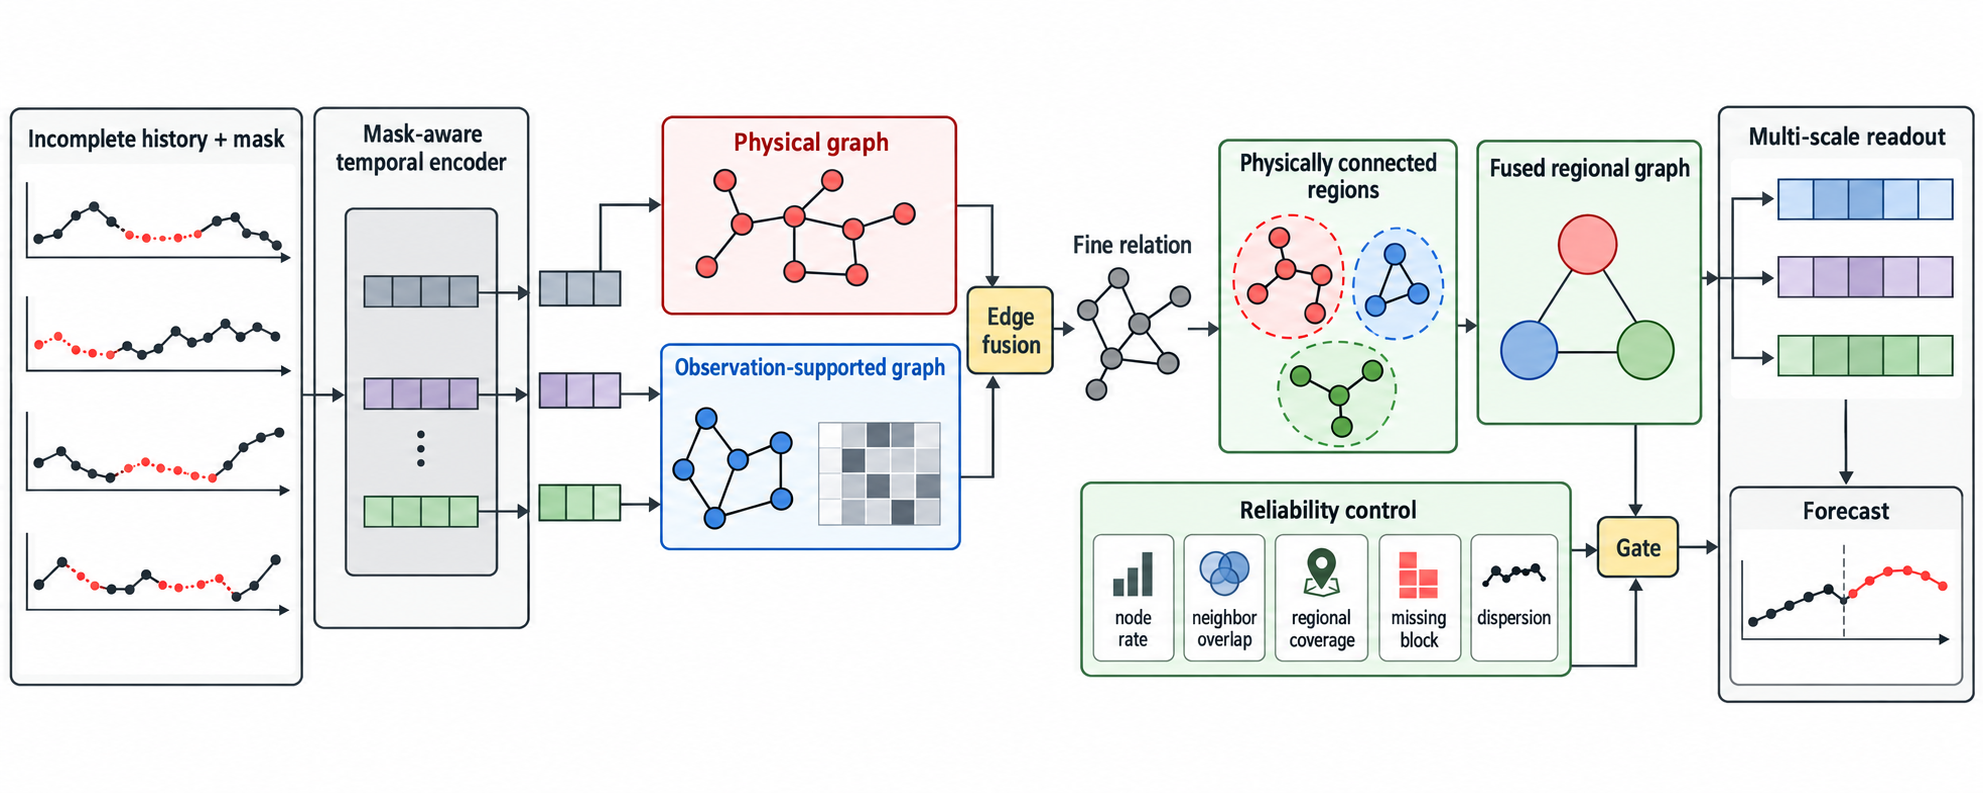
\includegraphics[width=0.98\textwidth]{figures/mr_msgf_overview.png}
  \caption{Overview of MR-MSGF. A mask-aware encoder forms temporal states from incomplete history. A co-observation-supported graph is fused with the physical graph before physically connected regional coarsening. Reliability evidence regulates regional residual injection and multi-scale readout.}
  \label{fig:mrmsgf-overview}
\end{figure*}

\subsection{Observation-Supported Relation Fusion}

The encoder produces history features $E\in\mathbb{R}^{T\times N\times d}$. We obtain a window-specific node representation by masked pooling:
\begin{equation}
u_i=\frac{\sum_t\bar M_{t,i}E_{t,i}}{\sum_t\bar M_{t,i}+\epsilon}.
\end{equation}
The observation-supported score combines learned similarity and co-observation:
\begin{align}
s_{ij}&=\frac{(W_qu_i)^\top(W_ku_j)}{\sqrt d},\\
\tilde{s}_{ij}&=s_{ij}+\operatorname{softplus}(\beta)\log(q_{ij}+\epsilon).
\end{align}
For each node, we retain the top-$k$ entries of $\tilde{s}_{ij}$, apply a row softmax, add self-loops, and row-normalize to obtain $A^{\obs}$. The logarithmic term is a soft evidence penalty: an edge with little joint observation is discouraged before sparsification, without imposing a hard correlation rule.

The physical graph is normalized as $\bar A^{\phy}=\norm(A^{\phy}+I)$. A learned edge gate then forms the fine relation:
\begin{align}
g_{ij}&=\sigmoid\!\left(\psi_g([r_i,r_j,q_{ij},\bar A^{\phy}_{ij},A^{\obs}_{ij}])\right),\\
A^{\fine}&=\norm\!\left(g\odot\bar A^{\phy}+(1-g)\odot A^{\obs}\right).
\end{align}
Thus, both physical structure and observation-supported relations participate in a prediction-driven fusion.
The gate is intentionally edge-specific rather than a global mixing coefficient. A physical neighbor can be trusted when observation support is scarce, while an observation-supported edge can dominate when the current window contains enough joint evidence to reveal dynamic dependence beyond physical proximity.

\subsection{Reliability-Controlled Regional Context}

We construct a fixed hard assignment $S\in\{0,1\}^{N\times K}$ only from the physical graph. Each region is seeded by high physical degree and expanded through positive physical affinity until a pre-defined maximum size is reached. This produces physically connected local regions rather than unconstrained latent clusters. With $n_k=\sum_iS_{ik}$, the fine state, regional state, and coarse relation are
\begin{align}
Z^{\fine}_{\ell}&=\operatorname{ELU}(A^{\fine}H_{\ell}W_f+H_{\ell}W_s),\\
H^{\reg}_{\ell,k}&=\frac{1}{n_k}\sum_iS_{ik}Z^{\fine}_{\ell,i},\\
A^{\coarse}&=\norm(S^\top A^{\fine}S).
\end{align}
Regional propagation and lifting are
\begin{align}
Z^{\reg}_{\ell}&=\operatorname{ELU}(A^{\coarse}H^{\reg}_{\ell}W_c+H^{\reg}_{\ell}W_r),\\
Z^{\coarse}_{\ell}&=SZ^{\reg}_{\ell}.
\end{align}
Coarsening after fine-scale fusion preserves dynamic observation-supported relations before regional aggregation, whereas coarsening from only the physical or observation graph would discard one source of evidence.

For node $i$, let $\bar q_i=\sum_j\bar A^{\phy}_{ij}q_{ij}$ be physical-neighbor co-observation, $\rho_i=\sum_kS_{ik}n_k^{-1}\sum_jS_{jk}r_j$ be regional coverage, $b_i$ be the longest missing block divided by $T$, and $\delta_{i,\ell}$ be normalized within-region dispersion. The regional gate is
\begin{align}
\alpha_{i,\ell}=\sigmoid\big(&\psi_\alpha([r_i,\bar q_i,\rho_i,b_i,\delta_{i,\ell}])\\
&+\gamma^\top[1-r_i,1-\bar q_i,\rho_i-1,b_i,-\delta_{i,\ell}]\big).
\end{align}
The finest representation becomes
\begin{equation}
\widetilde B_{0,\ell}=Z^{\fine}_{\ell}+\alpha_{\ell}\odot\big(Z^{\coarse}_{\ell}W_p\big),
\end{equation}
while $\widetilde B_{s,\ell}=B_{s,\ell}$ for $s>0$. We also bias the multi-scale readout score by reliability evidence:
\begin{equation}
e_{s,\ell,i}=e^{\mathrm{repr}}_{s,\ell,i}+w_{s,\ell}^\top[r_i,\bar q_i,\rho_i,b_i].
\end{equation}
Training minimizes masked forecasting MAE,
\begin{equation}
\mathcal{L}_{\mathrm{pred}}=\frac{\sum M^Y\odot|\hat Y-Y|}{\sum M^Y},
\end{equation}
where $M^Y$ excludes unavailable future targets. We do not use reconstruction, graph, or clustering auxiliary losses.
The gate is not interpreted as calibrated uncertainty. It is a forecasting-oriented control variable that decides whether regional context should be added for a node at a temporal level. This design keeps the added branch lightweight while making regional messages conditional on missingness evidence rather than unconditional smoothing.

\section{Experiments}

\subsection{Settings}

We evaluate on METR-LA traffic speeds and AQI36 air quality. All experiments forecast 12 steps from 24 historical steps. For METR-LA, Point and Block-T masks are applied only to the historical input; future targets are evaluated on valid, unmasked raw values. Point masks simulate independent random sensor-value loss, while Block-T masks simulate contiguous temporal outages. AQI36 retains its native validity mask and adds optional Point masks on top. Each condition uses five paired mask seeds, and compared models share the same input masks. The model is trained only with the masked forecasting loss in Eq.~(16), without imputation or graph auxiliary losses. HD-TTS-AMP is the main reference. METR-LA also includes BiTGraph connected to the common data, mask, and evaluation interface; because its original training schedule differs from HD-TTS, we interpret it only as a unified-protocol comparison.

\subsection{Main Results}

Table~\ref{tab:metr-main} reports METR-LA results. MR-MSGF lowers MAE over HD-TTS-AMP in all tested Block-T and Point settings. It also improves RMSE under Block-T 30\%/50\% and Point 30\%/50\%. At Block-T 70\%, MR-MSGF still improves MAE but has slightly worse RMSE, indicating that the benefit is not cross-metric consistent under extreme missingness.

\begin{table}[!t]
\centering
\small
\caption{METR-LA results over five paired mask seeds. Lower is better; the best result within each condition is in bold.}
\label{tab:metr-main}
\resizebox{\columnwidth}{!}{%
\begin{tabular}{l c l c c}
\toprule
Mask & Rate & Method & MAE & RMSE \\
\midrule
Block-T & 30\% & HD-TTS-AMP & $3.2281 \pm 0.0108$ & $6.6036 \pm 0.0126$ \\
& & BiTGraph & $3.8232 \pm 0.0110$ & $7.8839 \pm 0.0373$ \\
\rowcolor{gray!14} & & \ours & \best{3.1997 \pm 0.0159} & \best{6.5840 \pm 0.0485} \\
\cmidrule(lr){2-5}
& 50\% & HD-TTS-AMP & $3.3546 \pm 0.0126$ & $6.8780 \pm 0.0215$ \\
& & BiTGraph & $3.9729 \pm 0.0180$ & $8.1905 \pm 0.0458$ \\
\rowcolor{gray!14} & & \ours & \best{3.3079 \pm 0.0195} & \best{6.8154 \pm 0.0554} \\
\cmidrule(lr){2-5}
& 70\% & HD-TTS-AMP & $3.4650 \pm 0.0103$ & \best{7.0927 \pm 0.0421} \\
& & BiTGraph & $4.1363 \pm 0.0132$ & $8.4812 \pm 0.0306$ \\
\rowcolor{gray!14} & & \ours & \best{3.4458 \pm 0.0102} & $7.1088 \pm 0.0384$ \\
\midrule
Point & 30\% & HD-TTS-AMP & $3.1048 \pm 0.0074$ & $6.3592 \pm 0.0154$ \\
& & BiTGraph & $3.6374 \pm 0.0124$ & $7.5260 \pm 0.0377$ \\
\rowcolor{gray!14} & & \ours & \best{3.0764 \pm 0.0118} & \best{6.3091 \pm 0.0447} \\
\cmidrule(lr){2-5}
& 50\% & HD-TTS-AMP & $3.1598 \pm 0.0112$ & $6.4755 \pm 0.0215$ \\
& & BiTGraph & $3.6938 \pm 0.0049$ & $7.6577 \pm 0.0289$ \\
\rowcolor{gray!14} & & \ours & \best{3.1409 \pm 0.0068} & \best{6.4564 \pm 0.0289} \\
\bottomrule
\end{tabular}
}
\end{table}

\subsection{Cross-Domain and Horizon Analysis}

AQI36 provides a cross-domain stress test with native missingness. Table~\ref{tab:aqi} shows that MR-MSGF is worse than HD-TTS-AMP under native missingness, improves both metrics with an additional 25\% Point mask, and lowers MAE but raises RMSE with an additional 50\% Point mask. We therefore treat AQI36 as mixed evidence rather than claiming dataset-independent gains.

\begin{table}[t]
\centering
\small
\caption{AQI36 cross-domain results over five seeds.}
\label{tab:aqi}
\resizebox{\columnwidth}{!}{%
\begin{tabular}{l l c c}
\toprule
Condition & Method & MAE & RMSE \\
\midrule
Native & HD-TTS-AMP & \best{30.4839 \pm 0.5849} & \best{49.3332 \pm 1.4069} \\
& \ours & $30.7269 \pm 0.2392$ & $49.8879 \pm 0.9287$ \\
\cmidrule(lr){1-4}
Native+P25 & HD-TTS-AMP & $31.2034 \pm 0.6894$ & $50.3712 \pm 1.0346$ \\
& \ours & \best{31.1169 \pm 0.4161} & \best{50.3325 \pm 0.7815} \\
\cmidrule(lr){1-4}
Native+P50 & HD-TTS-AMP & $31.7359 \pm 0.4956$ & \best{50.4029 \pm 1.2035} \\
& \ours & \best{31.6451 \pm 0.7093} & $50.5270 \pm 1.3859$ \\
\bottomrule
\end{tabular}
}
\end{table}

We also decompose METR-LA Block-T checkpoints by prediction horizon. At 50\% missingness, MR-MSGF lowers both MAE and RMSE at horizons 3, 6, and 12. At 70\% missingness, it slightly lowers MAE at all three horizons but raises RMSE at each horizon, matching the aggregate result in Table~\ref{tab:metr-main}. The extreme-missingness gain is therefore concentrated on average error rather than large-error control.

\begin{table}[t]
\centering
\small
\caption{METR-LA Block-T horizon decomposition.}
\label{tab:horizon}
\resizebox{\columnwidth}{!}{%
\begin{tabular}{c c c c}
\toprule
Rate & Horizon & HD-TTS-AMP MAE/RMSE & \ours{} MAE/RMSE \\
\midrule
50\% & 3 & $3.1319/6.2557$ & \best{$3.0750/6.1586$} \\
50\% & 6 & $3.3787/6.9274$ & \best{$3.3333/6.8715$} \\
50\% & 12 & $3.6532/7.6045$ & \best{$3.6195/7.5840$} \\
70\% & 3 & $3.2773/\best{6.5703}$ & $\best{3.2520}/6.5811$ \\
70\% & 6 & $3.4777/\best{7.1235}$ & $\best{3.4667}/7.1568$ \\
70\% & 12 & $3.7302/\best{7.7343}$ & $\best{3.7186}/7.7618$ \\
\bottomrule
\end{tabular}
}
\end{table}

\subsection{Ablation and Diagnostics}

Table~\ref{tab:ablation} isolates the Block-T 50\% mechanisms. The full model is best on both metrics. Removing the co-observation score penalty, the reliability gate, or the readout bias all hurts performance, and using only one fine relation source is weaker than the fused graph. This supports the central design choice: co-observation-guided relation fusion and reliability-controlled regional context are complementary.

\begin{center}
\refstepcounter{table}\label{tab:ablation}
\small
\textbf{Table~\thetable.} METR-LA Block-T 50\% ablation over five paired seeds.
\resizebox{\columnwidth}{!}{%
\begin{tabular}{l c c}
\toprule
Variant & MAE & RMSE \\
\midrule
HD-TTS-AMP & $3.3546 \pm 0.0126$ & $6.8780 \pm 0.0215$ \\
Physical only & $3.3292 \pm 0.0118$ & $6.8605 \pm 0.0490$ \\
Observation only & $3.3348 \pm 0.0161$ & $6.8874 \pm 0.0587$ \\
Fused graph & $3.3176 \pm 0.0111$ & $6.8288 \pm 0.0455$ \\
No $q_{ij}$ penalty & $3.3149 \pm 0.0200$ & $6.8327 \pm 0.0547$ \\
No rel. gate & $3.3136 \pm 0.0105$ & $6.8395 \pm 0.0420$ \\
No readout bias & $3.3298 \pm 0.0249$ & $6.8512 \pm 0.0375$ \\
\rowcolor{gray!14} Full \ours & \best{3.3079 \pm 0.0195} & \best{6.8154 \pm 0.0554} \\
\bottomrule
\end{tabular}
}
\end{center}

As a diagnostic, the Pearson correlation between non-diagonal co-observation rates and physical-edge gates $g_{ij}$ is $-0.4051$ across 10 full-model checkpoint evaluations. Since larger $g_{ij}$ assigns more weight to the physical graph, this negative association is consistent with greater use of observation-supported relations when co-observation is available, though it is not causal evidence. Table~\ref{tab:efficiency} shows that MR-MSGF adds 7.7\% parameters while keeping measured inference time at a comparable scale.

\begin{center}
\refstepcounter{table}\label{tab:efficiency}
\small
\textbf{Table~\thetable.} Post-hoc efficiency statistics.
\begin{tabular}{l c c}
\toprule
Method & Params & Test batch time (s) \\
\midrule
HD-TTS-AMP & 378,351 & $0.2692 \pm 0.0907$ \\
\ours & 407,447 & $0.2672 \pm 0.1065$ \\
\bottomrule
\end{tabular}
\end{center}

\section{Conclusion}

MR-MSGF forecasts from incomplete spatial history by estimating a co-observation-regularized relation graph, fusing it with physical structure, and injecting regional context through a reliability gate. The strongest evidence is on METR-LA missing-history forecasting, where MR-MSGF consistently improves MAE and improves RMSE except under extreme Block-T missingness. The mixed AQI36 results suggest that cross-domain stability remains an important limitation and a useful direction for future validation.

\bibliographystyle{../template/IEEEbib}
\bibliography{references}

\end{document}
